\documentclass[preprint2]{aastex6}
\newcommand{\vdag}{(v)^\dagger}
\newcommand\aastex{AAS\TeX}
\newcommand\latex{La\TeX}

\usepackage{graphicx}
\usepackage{txfonts}
\usepackage{color}

\usepackage{hyperref}
\usepackage{aas_macros}
\usepackage{natbib}
\bibpunct{(}{)}{;}{a}{}{,}

%% AASTeX 6.0 supports the ability to suppress the names and affiliations
%% of some authors and displaying them under a "collaboration" banner to
%% minimize the amount of author information that to be printed.  This 
%% should be reserved for articles with an extreme number of authors.
%%
%% Mark up commands to limit the number of authors on the front page.
\AuthorCallLimit=1
%% Will only show Schwarz & Muench since Schwarz and Muench
%% are in the same \author call. 
\fullcollaborationName{The Friends of AASTeX Collaboration}
%% will print the collaboration text after the shortened author list.
%% These commands have to COME BEFORE the \author calls.
%%
%% Note that all of these author will be shown in the published article.
%% This feature is meant to be used prior to acceptance to make the
%% front end of a long author article more manageable.
%% Use \allauthors at the manuscript end to show the full author list.

%% The following command can be used to set the latex table counters.  It
%% is needed in this document because it uses a mix of latex tabular and
%% AASTeX deluxetables.  In general it should not be needed.
%\setcounter{table}{1}

%%%%%%%%%%%%%%%%%%%%%%%%%%%%%%%%%%%%%%%%%%%%%%%%%%%%%%%%%%%%%%%%%%%%%%%%%%%%%%%%
%%
%% The following commented section outlines numerous optional output that
%% can be displayed in the front matter or as running meta-data.
%%
%% You can insert a short comment on the title page using the command below.
%% \slugcomment{Not to appear in Nonlearned J., 45.}
%%
%% If you wish, you may supply running head information, although
%% this information may be modified by the editorial offices.
%%\shorttitle{\aastex sample article}
%%\shortauthors{Schwarz et al.}
%%
%% You can add a light gray and diagonal water-mark to the first page 
%% with this command:
%% \watermark{text}
%% where "text", e.g. DRAFT, is the text to appear.  If the text is 
%% long you can control the water-mark size with:
%% \setwatermarkfontsize{dimension}
%% where dimension is any recognized LaTeX dimension, e.g. pt, in, etc.
%%
%%%%%%%%%%%%%%%%%%%%%%%%%%%%%%%%%%%%%%%%%%%%%%%%%%%%%%%%%%%%%%%%%%%%%%%%%%%%%%%%

%% This is the end of the preamble.  Indicate the beginning of the
%% paper itself with \begin{document}.

\begin{document}

\title{The density of an accretion disk atmosphere}

\author{Agata R\'o\.za\'nska\altaffilmark{1}, Dominik Gronkiewicz\altaffilmark{1}, 
Matteo Guianazzi\altaffilmark{2}, Bartosz Be\l dycki\altaffilmark{1}, Tek P. Adhikari\altaffilmark{1}, Swayamtrupta Panda\altaffilmark{1}, Alex Markowitz\altaffilmark{1}, Krzysztof Hryniewicz\altaffilmark{1}, Bo\.zena Czerny\altaffilmark{3}, 
Jiri Svoboda\altaffilmark{4}, Michal Dovciak\altaffilmark{4}
}
%\fo

\altaffiltext{1}{Copernicus Astronomical Center, Bartycka 18, 00-716 Warszawa, Poland, agata@camk.edu.pl}
\altaffiltext{2}{ESTEC, Keplerlaan 1 2201AZ Noordwijk, The Netherlands}
\altaffiltext{3}{Center for Theoretical Physics, Al. Lotnik{\'o}w 32/46, 02-680 Warsaw, Poland}
\altaffiltext{4}{Astronomical Institute of the Czech Academy of Sciences, Boční II 1401
141 00 Praha 4, Czech Republic}

\begin{abstract}

In this paper we derive disk denstities for various heating mechanizms. 
\end{abstract}

\keywords{accretion,accretion disks --- stars:neutron --- X-rays:general}

\section{Introduction}

Accretion disk atmospheres are a gas reservoir where radiation interacts with matter including 
strong irradiation from external X-ray source. They may undergo the influence of radiation forces due to different processes i.e. Compton scattering, photoionization or line transition. On the other hand, 
it is believed that accretion disk atmospheres are heated by typical viscosity mechanism which may be a magnetic field reconection \citep{1992-ToutPringle,1999-BalbusPapaloizou}. Atmospheres may be thermally unstable giving the raise to multi-phase medium \citep{} or gas outflow in the form of 
ionized wind \citep{}

We present the disk densities which outcome from vertical simulations of accretin disk structure 
taking into accout diffeent processes responsible for accretions. 
In the first step, we assume that viscous tourque is proportional to the gas pressure only. 
In the second step we compare those results to the radiative pressure dominated disks. 
Furthermore, we derive densities when viscous tourque is proportional to the total pressure. 
In the last step we assume that the gas in the disk is heated by magnetic reconnection 
following \citet{Gronkiewicz2018}. 

We consider different masses and spins of black holes and different. 



\section{Vertical disk structure}
\label{sec:mod}

We compute the vertical structure of optically thick accretion disk parametrized by black hole 
mass $M_{\rm BH}$, accretion rate $\odot m$ and black hole spin $a$ for all possible distances
ranging from inermost stable circular orbit (ISCO) up to outer radius of the order of thousand 
gravitational radii.   

\section{Model parameters}
\label{sec:param}

SMBH
IMBH
GBHC
rozne tempa akrecji dwa rozne 

Rozne torque propotionality:
\begin{itemize}
\item Pgas
\item Prad
\item Ptot 
\item Magnetic reconection (Dominik)
\end{itemize}

Different opacities:
-scattering and absorption 

GR in vertical structure and not 

\section{Results}


\section{Comparison with observations}
\label{sec:source}

From BLR region 

From outflows including WA 

From Reverberation mapping 

From lines 

From other variability mehtod 

\section{Discussion}
\label{sec:data}


Kallman (find the paper)
Tomsick (recent paper) 

To complete literature. 


\begin{figure*}
 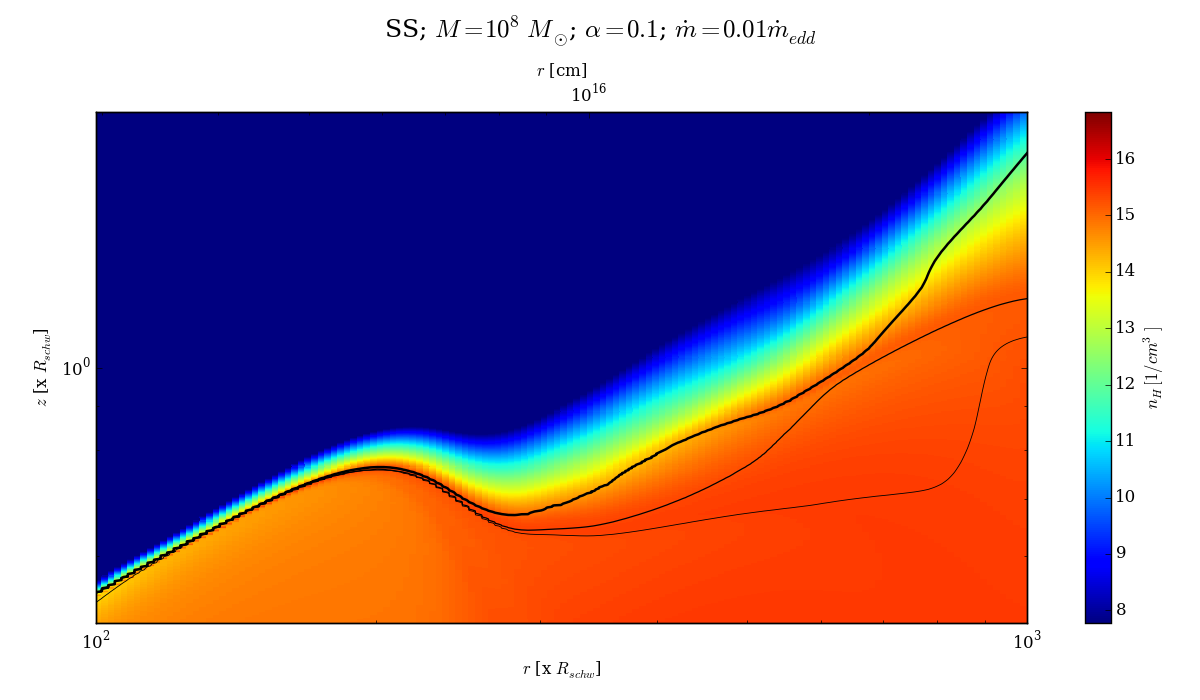
\includegraphics[scale=0.62]{plot_ss_r100.png}
 \caption{The density from the accretion disk predicted from the vertically integrated SS73 model for AGN case.  
 Black solid lines denote places with the same optical depth computed with diffution approximation of radiative transfer.}
 \label{fig:counts*}
\end{figure*}



\section{Conclusions}
\label{sec:results}


\begin{table}
\begin{center}
\begin{tabular}{lll}
\hline 
Parameter & Value & Unit \\ 
\hline\hline
$\chi^2/dof$ & 1344/1245  & -- \\
$F_{\rm X}$(2-10 keV) & 4.36 $\times10^{-12}$ & erg$\cdot$s$^{-1}\cdot$cm$^{-2}$\\
$F_{\rm X}$(0.3-30 keV) & 6.83 $\times10^{-12}$ & erg$\cdot$s$^{-1}\cdot$cm$^{-2}$\\
$D=10/\sqrt{N}$ & 3.41$^{+0.11}_{-0.10}$ & Mpc\\ 
$ L_{\rm X}$(0.3-30 keV)  & 9.59 $\times10^{39}$& erg$\cdot$s$^{-1}$\\ 
\hline 
\end{tabular}
\end{center}
\end{table}


\section{Discussion}
\label{sec:sum}


\section*{Acknowledgments}

This research was supported by Polish National Science 
Center grants No. 2015/17/B/ST9/03422, 2015/18/M/ST9/00541, and 2016/21/N/ST9/03311.  

\bibliographystyle{aasjournal}
\bibliography{disks}

\end{document}

%%%%%%%%%%%%%%%%%%%%%%%%%%%%%%%%
%%%%%%%%%%%%%%%%%%%%%%%%%%%%%%%%
